\chapter{Message Passing}%
\label{chap:07}

\section{Dynamic Programming on Trees}
In many applications in computer vision we want to model
connectivity. Consider the segmentation of blood vessels in a
lung. These vessels form a tree and thus it is natural to pose a
connectivity constraint in a segmentation task. For example, this
leads to the connections of previously unconnected regions which in
turn reduces the noise in the computed segmentation.

Trees are also a very natural choice for modelling hierarchies. For
instance, in cell segmentation, one can represent the segmented cells
in a tree structure where children correspond to the individual parts
of a ``clumped'' cell, see also the Figure below.

We can also model (simple) constellations; applications are facial
feature detection in images. Here, the parts of a face (eyes, nose,
mouth etc.) are modelled in a tree structure where the edges can be
interpreted as springs in a star configuration to the nose, see the
Figure below. Extending these springs or posing them in certain
positions that do not make sense has a high cost, and thus, plausible
configurations that correspond to realistic facial features correspond
to low costs.
\begin{figure}[htpb]
  \begin{subfigure}[c]{0.5\textwidth}
    \centering
    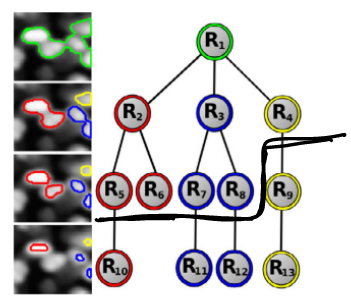
\includegraphics[width=0.7\linewidth]{Figures/tree-cells}
  \end{subfigure}%
  \begin{subfigure}[c]{0.5\textwidth}
    \centering
    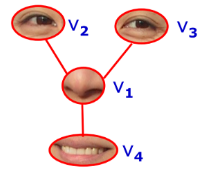
\includegraphics[width=0.7\linewidth]{Figures/tree-face}
  \end{subfigure}
  \caption{Two example of how trees can be used to model hierarchies
    and simple constellations in computer vision applications.}
\end{figure}

%%% Local Variables:
%%% mode: latex
%%% TeX-master: "../main"
%%% End:
